% Example paper. Replace the content, keep the structure:
% one file per section and one sentence per line (see docs/writing-guidelines.md).
\documentclass[11pt]{article}

\usepackage[utf8]{inputenc}
\usepackage[T1]{fontenc}
\usepackage[margin=2.5cm]{geometry}
\usepackage{amsmath,amssymb}
\usepackage{graphicx}
\usepackage{booktabs}
\usepackage{tikz}
\usepackage[hidelinks]{hyperref}

\graphicspath{{figures/}}

\title{An Example Paper Built with texops}
\author{First Author \and Second Author}
\date{}

\begin{document}

\maketitle

\begin{abstract}
This document is a minimal example of a paper written with texops.
It shows sections split into files, a figure, a table, an equation and citations.
Every change proposed in a pull request is compiled automatically and rendered as a visual diff.

\end{abstract}

% !TEX root = ../main.tex
\section{Introduction}
\label{sec:introduction}

Scientific papers are rarely written by a single person.
A typical manuscript goes through several rounds of drafting, internal review and revision before it is submitted, and often through more rounds after the reviewers' comments arrive.
Each round involves co-authors, advisors or collaborators who need to read the current version, suggest changes and check that their suggestions were addressed.

In practice, this collaboration is often managed in an ad hoc way.
Co-authors exchange files by e-mail, rename them with dates or initials, and merge contributions by hand.
Comments are scattered across e-mail threads, annotated PDFs and messaging applications.
As a result, it becomes hard to know which version is the latest, who changed what, and whether a given comment has already been handled.

Online editors reduce some of these problems by keeping a single shared copy of the document.
However, they usually record changes as a continuous history rather than as reviewable units, and they tie the writing process to a specific platform.
Moreover, differences in compiler versions or installed packages between co-authors can still produce documents that look different on each machine.

Software development faced similar problems long ago and addressed them with version control, code review and continuous integration.
In that setting, every change is proposed as a pull request, discussed line by line, built automatically in a controlled environment and merged only after approval.
These practices make the history of a project explicit and the review of each change systematic.

texops applies the same practices to academic writing.
The paper is kept as \LaTeX{} source code~\cite{lamport1994latex} in a Git repository, and every change goes through a pull request.
A continuous integration pipeline compiles the paper inside a Docker image, so every author and reviewer obtains exactly the same PDF.
For each pull request, the pipeline also produces a visual diff with latexdiff~\cite{latexdiff}, in which removed text is marked in red and added text in blue.
Reviewers can therefore follow the evolution of the paper from their browser, without installing any software.

The main contributions of this example paper are the following:
\begin{itemize}
  \item a reproducible writing environment, shared by the editor, local builds and continuous integration;
  \item a review workflow in which every change is available both as a line diff of the source and as a visual diff of the PDF;
  \item a set of writing conventions, such as one sentence per line, that keep changes small and easy to review.
\end{itemize}

The rest of this paper is organized as follows.
Section~\ref{sec:method} describes the method, Section~\ref{sec:results} presents the results and Section~\ref{sec:conclusion} concludes.

% !TEX root = ../main.tex
\section{Method}
\label{sec:method}

Given a training set $\mathcal{D} = \{(x_i, y_i)\}_{i=1}^{n}$, a model $h_\theta$ is fitted by minimizing the empirical risk
\begin{equation}
  \hat{\theta} \in \arg\min_{\theta} \frac{1}{n} \sum_{i=1}^{n} \ell\big(h_\theta(x_i), y_i\big).
  \label{eq:erm}
\end{equation}

Figure~\ref{fig:pipeline} summarizes the writing workflow.

\begin{figure}[ht]
  \centering
  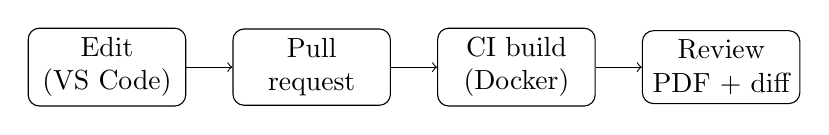
\begin{tikzpicture}[node distance=2.6cm, every node/.style={draw, rounded corners, minimum width=2cm, minimum height=0.8cm, align=center}]
    \node (edit) {Edit\\(VS Code)};
    \node (pr) [right of=edit] {Pull\\request};
    \node (ci) [right of=pr] {CI build\\(Docker)};
    \node (review) [right of=ci] {Review\\PDF + diff};
    \draw[->] (edit) -- (pr);
    \draw[->] (pr) -- (ci);
    \draw[->] (ci) -- (review);
  \end{tikzpicture}
  \caption{Writing workflow.}
  \label{fig:pipeline}
\end{figure}

\section{Results}
\label{sec:results}

Table~\ref{tab:results} shows illustrative numbers.

\begin{table}[ht]
  \centering
  \caption{Illustrative results.}
  \label{tab:results}
  \begin{tabular}{lcc}
    \toprule
    Model & Precision & Recall \\
    \midrule
    Baseline & 0.81 & 0.77 \\
    Proposed & 0.88 & 0.85 \\
    \bottomrule
  \end{tabular}
\end{table}

\section{Conclusion}
\label{sec:conclusion}

This example demonstrated the structure expected by texops.
Replace these files with your own content and keep one sentence per line.


\bibliographystyle{plain}
\bibliography{references}

\end{document}
